\documentclass[landscape,fontscale=1,margin=0.2cm,paperwidth=60truecm, paperheight=34truecm,debug]{baposter}
\usepackage{multirow}
\begin{document}

\begin{poster}{
  headerheight=60pt,
  columns=4,
  background=plain,
%   linewidth=0.5pt,
  borderColor=orange!70,
  textborder=rectangle,
  headershade=plain,
  headerColorOne=orange!80,
  headershape=smallrounded,
  boxheaderheight=1.5em,
  headerfont={},
  boxColorOne=white,
  bgColorOne=darkgray,
  bgColorTwo=blue!60,
}{}{\Large{\color{white}{Single Cycle Datapath}}}{}{d}

%%%%%%%%%%%%%%%%%%%%%%%%%%%%%%%%%%%%%%%%%%%%%%%%%%%%%%%%%%%%%%%%%%%%%%%%%%%%%%
\begin{posterbox}[column=0]{Datapath Elements}
\begin{description}
\item[Program counter (PC)] an incrementing counter that keeps track of the memory address of the instruction that is to be executed next.
\item[Memory address register (MAR)] holds the address of a memory block to be read from or written to.
\item[Memory data register (MDR)] a two-way register that holds data fetched from memory (and ready for the CPU to process) or data waiting to be stored in memory
\item[Instruction register (IR)] a temporary holding ground for the instruction that has just been fetched from memory
\item[Control unit (CU)] decodes the program instruction in the IR, selecting machine resources such as a data source register and a particular arithmetic operation, and coordinates activation of those resources
\item[Arithmetic logic unit (ALU)] performs mathematical and logical operations
\end{description}
\end{posterbox}
\begin{posterbox}[column=0,below=auto,textborder=rounded]{Fetch Execute Cycle}
\begin{center}
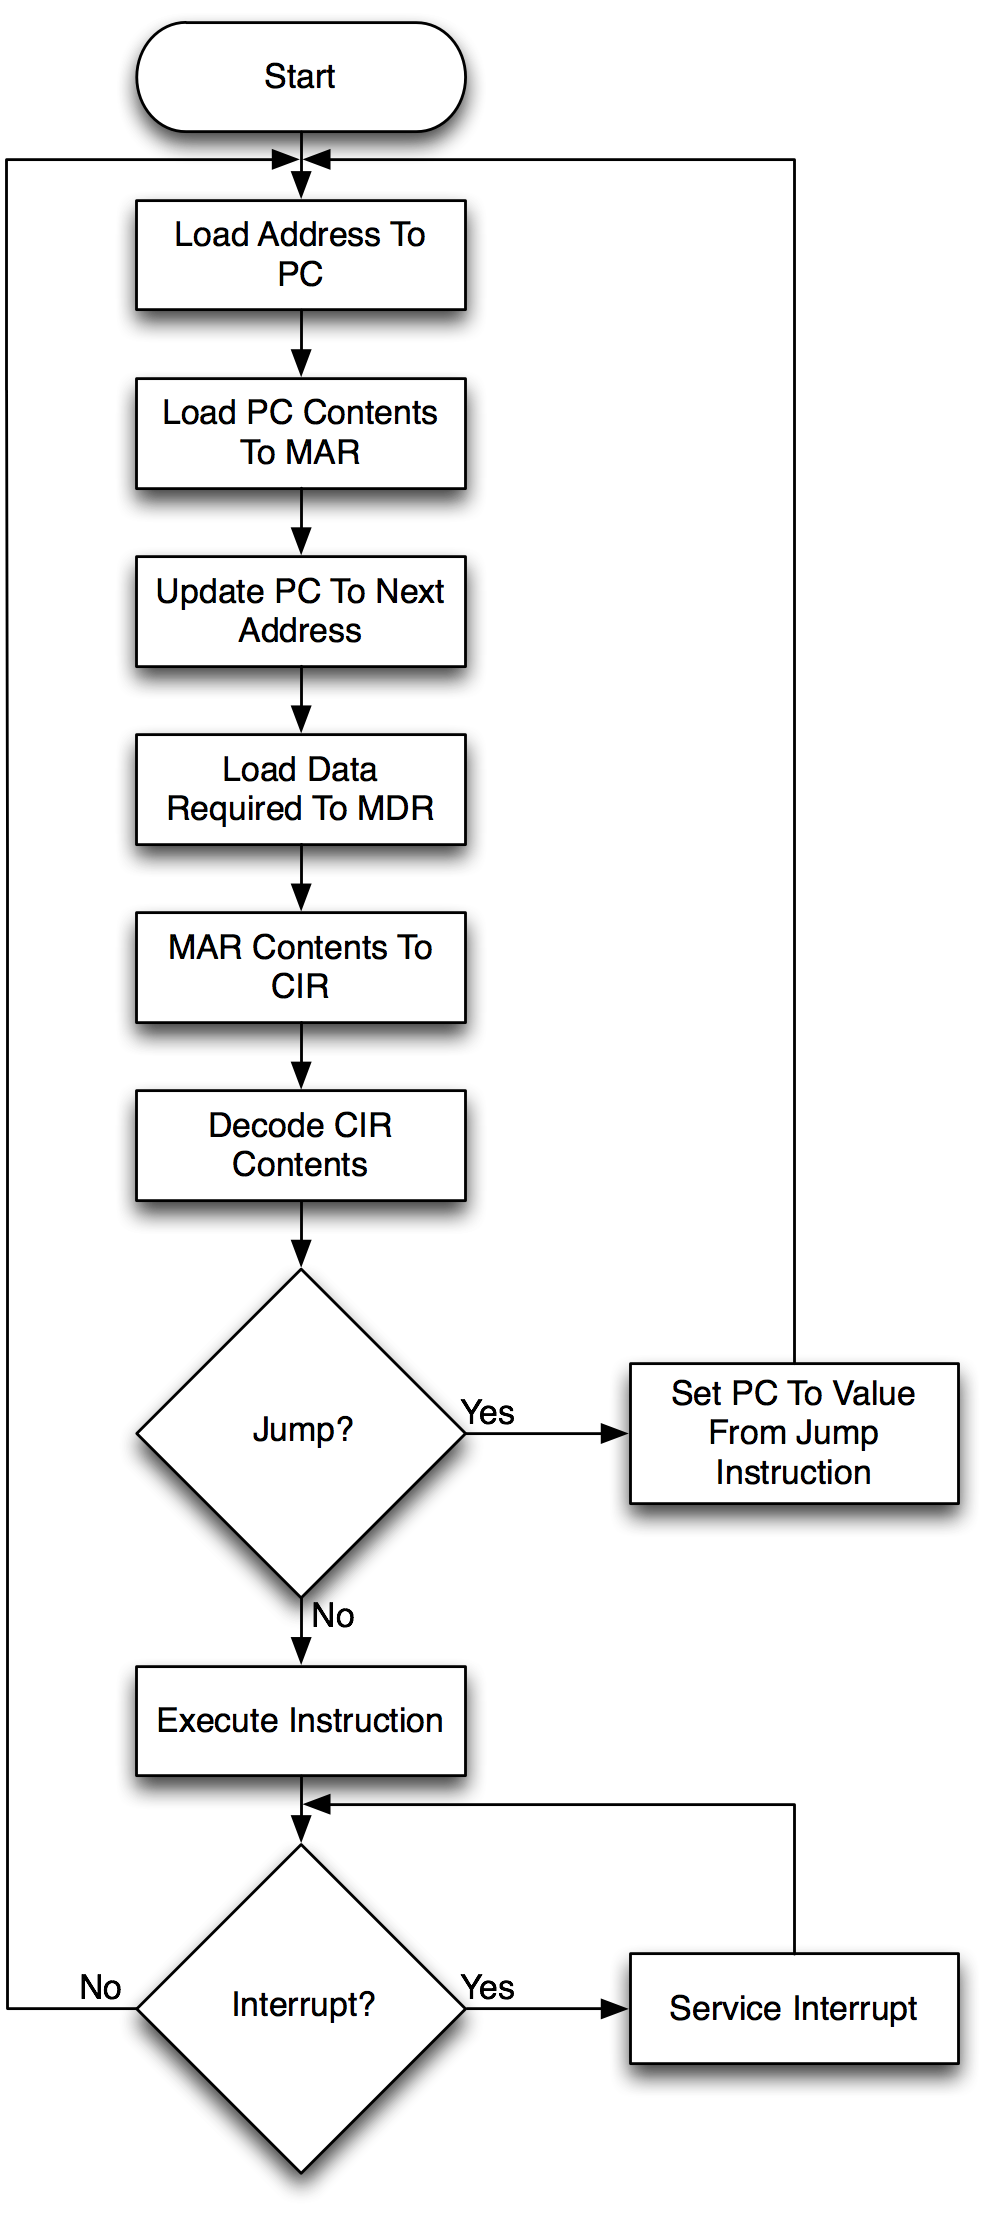
\includegraphics[scale=0.5]{fetchExCycle.png}
\end{center}
\end{posterbox}
\begin{posterbox}[column=1]{R-Type Instruction Classes}
\begin{center}
\begin{tabular}{|l |c|c|c|c|c|c|}
\hline
Field & 0 & rs & rt & rd & ShiftAmt & funct\\\hline
Bit Positions &31:26&25:21&20:16&15:11&10:6&5:0\\\hline
\end{tabular}
\end{center}
\end{posterbox}

\begin{posterbox}[column=1,below=auto]{Some R-Type Math Instructions}
\begin{center}
\begin{tabular}{|c|c|c|c|}
\hline
instruction & opcode & function & func base 2\\\hline
add & 0 & 32 & 100000 \\\hline
sub & 0 & 34 & 100010 \\\hline
and & 0 & 36 & 100100 \\\hline
or & 0 & 37& 100101 \\\hline
slt & 0 & 42 & 101010 \\\hline

\end{tabular}
\end{center}
\end{posterbox}
\begin{posterbox}[column=1,below=auto]{R-Type Example}
\begin{center}
\begin{tabular}{|c|c|c|c|c|c|}
\hline
Opcode & rs & rt & rd & ShiftAmt & funct\\\hline
add & \$17 & \$18 & \$9 & N/A & 32\\\hline
000000 & 10001 & 10010 & 01001 & 00000 & 100000\\\hline
6 bits & 5 bits & 5 bits & 5 bits & 5 bits & 6 bits\\\hline 
\end{tabular}
\end{center}
\end{posterbox}
\begin{posterbox}[column=1,below=auto]{R-Type in datapath}
\begin{center}
\begin{tikzpicture}
  \tikzstyle{mux} = [ trapezium,   draw,   
                    shape border rotate = 270, trapezium angle = 60,  
                    inner ysep=0pt, outer sep=1pt, inner xsep=1pt, 
                    text width = 3em, 
                    node distance=3cm, font=\large ]

 \node [mux] {0\\1};
\end{tikzpicture}
\end{center}
\end{posterbox}
\begin{posterbox}[column=2,textborder=rounded]{I-Type instruction classes}
\begin{center}
\begin{tabular}{|c|c|c|c|}
\hline
opcode & rs & rt & memory address offset\\\hline\hline
lw & \$17 & \$8 & 8\\\hline
100011 & 10001& 01000 & 0000 0000 0000 1000\\\hline\hline
sw & \$20 & \$16 & 44\\\hline
101011 & 10100 & 10000 & 0000 0000 0010 1100\\\hline
\end{tabular}
\\

\end{center}
\end{posterbox}
\begin{posterbox}[column=3,textborder=rounded]{ALU control lines}
\begin{center}
\begin{tabular}{|c|c|}
\hline
ALU control lines & Function\\\hline
0000 & AND\\\hline
0001 & OR\\\hline
0010 & add\\\hline
0110 & subtract\\\hline
0111 & set on less than\\\hline
1100 & NOR\\\hline
\end{tabular}
\end{center}
\end{posterbox}
%%%%%%%%%%%%%%%%%%%%%%%%%%%%%%%%%%%%%%%%%%%%%%%%%%%%%%%%%%%%%%%%%%%%
%%%%END POSTER
%%%%%%%%%%%%%%%%%%%%%%%%%%%%%%%%%%%%%%%%%%%%%%%%%%%%%%%%%%%%%%%%%%%
\end{poster}

\end{document}

